\documentclass[12pt,titlepage]{article}
\usepackage[table]{xcolor}
\usepackage{longtable}
\usepackage[utf8]{inputenc}
%Language of Document Elements like Figure or Table
\usepackage[english]{babel}
\usepackage[bookmarks]{hyperref}
\usepackage{pdfpages}
\usepackage{graphicx}
\usepackage{float}
\usepackage{array}
\usepackage{lipsum} 
\usepackage[justification=centering]{caption}
\usepackage{enumitem}
\usepackage{chngcntr}
\usepackage{lscape}
\usepackage{fancyhdr}
\usepackage{listings}
\usepackage[style=alphabetic, backend=biber]{biblatex}
\usepackage{dafny}
\usepackage{hyperref}
\usepackage{nameref}
\usepackage[margin=1in]{geometry}
 
%Each Section in a new Page
\let\oldsection\section
\renewcommand\section{\clearpage\oldsection}

%Set space around and between lists
\setlist[enumerate]{noitemsep, topsep=0cm}
\setlist[itemize]{noitemsep, topsep=0cm}

%Figure/Table Numbering style "Section Number.figure counter
\renewcommand{\thefigure}{\arabic{section}.\arabic{figure}}
\renewcommand{\thetable}{\arabic{section}.\arabic{table}}

%Reset figure/table counter after section change
\counterwithin{figure}{section}
\counterwithin{table}{section}

\hypersetup{
	colorlinks,
	linkcolor={black},
	citecolor={black},
	urlcolor={black}
}

%Syntax Highlighting
%\lstdefinestyle{dafny}{
%	language=dafny, 
%	basicstyle=\normalfont\ttfamily,
%	numbers=left,
%	numberstyle=\scriptsize,
%	stepnumber=1,
%	numbersep=8pt,
%	showstringspaces=false,
%	breaklines=true,
%	frame=lines,
%	backgroundcolor=\color{background}
%}

\colorlet{punct}{red!60!black}
\definecolor{background}{HTML}{EEEEEE}
\definecolor{delim}{RGB}{20,105,176}
\colorlet{numb}{magenta!60!black}

\lstdefinelanguage{json}{
	basicstyle=\normalfont\ttfamily,
	numbers=left,
	numberstyle=\scriptsize,
	stepnumber=1,
	numbersep=8pt,
	showstringspaces=false,
	breaklines=true,
	frame=lines,
	backgroundcolor=\color{background},
	literate=
	*{0}{{{\color{numb}0}}}{1}
	{1}{{{\color{numb}1}}}{1}
	{2}{{{\color{numb}2}}}{1}
	{3}{{{\color{numb}3}}}{1}
	{4}{{{\color{numb}4}}}{1}
	{5}{{{\color{numb}5}}}{1}
	{6}{{{\color{numb}6}}}{1}
	{7}{{{\color{numb}7}}}{1}
	{8}{{{\color{numb}8}}}{1}
	{9}{{{\color{numb}9}}}{1}
	{:}{{{\color{punct}{:}}}}{1}
	{,}{{{\color{punct}{,}}}}{1}
	{\{}{{{\color{delim}{\{}}}}{1}
	{\}}{{{\color{delim}{\}}}}}{1}
	{[}{{{\color{delim}{[}}}}{1}
	{]}{{{\color{delim}{]}}}}{1},
}



\newcommand{\todonl}[1]{\newline\textcolor{red}{TODO: #1}\PackageWarning{TODO:}{#1!}}
\newcommand{\todo}[1]{\textcolor{red}{TODO: #1}\PackageWarning{TODO:}{#1!}}

%Set Paragraph indent to null
\setlength{\parindent}{0pt}
% Smaler Table Space
\renewcommand{\arraystretch}{1.5}

\title{Visual Studio Code Integration for the Dafny Language and Program Verifier}
\author{Rafael Krucker, Markus Schaden}
\date{20.02.2017}

\pagestyle{fancy}
\lhead{BA Dafny}
\addbibresource{LITERATURVERZEICHNIS/bibliographie.bib}
\begin{document}
\pagenumbering{Roman} 



\includepdf{titlepage/titlepage}


\includepdf[pages={1-}]{section/TaskDescriptionBADafnyIDE}

\newpage
\tableofcontents
\newpage
\pagenumbering{arabic}

\section{Abstract}
The goal of this project was to integrate the Dafny programming language into Visual Studio Code. Emphasis was put into researching how Dafny programmers can be best supported during their work and how writing code can be made more productive.\newline 
Since Dafny offers built-in specification constructs, novel work is to provide tooling that makes using them easier. The most beneficial feature would have been to implement a generic, context aware proof obligation generator that continuously suggests specification constructs to the programmer. This approach was eventually discarded because it was deemed unfeasible to implement after some research had been done. Instead, situations were identified that arise often during programming, for example bound checking, and specific aid with specification constructs was implemented for them. Another helpful feature is the displaying of counter examples where code written does not satisfy the corresponding specification constructs, allowing quick discovery of edge cases and refinement of specification constructs.\newline 
Next to language specific features, standard IDE mechanisms allow for improvement regarding productivity. It was deemed paramount that the project implements the most common features such as go to definition and auto completion. This was achieved using the standard interfaces that Visual Studio Code provides, allowing programmers accessing these features in a well-established way.\newline
It is of concern that new users can get started quickly, so that the user base continuous to grow. To support this, automatic installation on all major platforms was implemented. The installation resolves all dependencies such as the Dafny pipeline itself. To further maximize portability, the plugin implements the language server protocol. This allows for writing IDE agnostic language analysis platforms, making the plugin usable in Visual Studio Code, and also integrable into some other IDEs with only minor adjustments.\newline
This project concluded with the implementation of a production ready integration of Dafny into Visual Studio Code. Continuous integration allowed for a user base of about 300 people at the end of the project, proofing that the plugin is robust and works across multiple environments. Dafny programmers are supported in their coding with standard IDE mechanisms and Dafny specific features. Next to making the experience of programming more productive, this lays the foundation of a contentiously growing Dafny community.\newline







\section{Management Summary}
Following the quickly growing digitalization of businesses and the therefor more complex applications being developed, two key points are gaining focus in today's IT landscape. The first one is the proven functional correctness of programs and the second one is the uprising of multi threaded applications. Writing multi threaded applications becomes much simples once the functional correctness is proven, thus it can be stated that proven functional correctness is a stepping stone towards the easier implementation of parallelism. Dafny is a programming language which tries to move the focus of writing correct code towards writing correct specification constructs, which is often easier. Applying this concept consistently should result in being able to turn business requirements into correct working implementations quicker as with traditional languages. The proven correlation between the time of discovering an error and the cost of fixing it also strongly advises writing software which is proven correctly as early in the life cycle of the product as possible. Even though using Dafny in business is compelling for these reasons, its usage is still not widespread, something which this project tries to change.\newline
The wide spread usage of a tool for programmers is mainly dictated by two factors, namely the burden of getting it to run and the support that it is able to offer the programmer. \newline
To address the first point, the plugin was developed for Visual Studio Code, an IDE running on all major platforms. It was also given an installation routine which resolves all dependencies on all platforms automatically after pressing one button. This also allows programmers that are not that familiar with the console to rapidly develop Dafny programs, something that was not possible given the tooling existing up until now. \newline
Regarding the second point, it was always paramount to offer as much help as possible to the programmer. This was done in two steps, the first one being implementing standard features that a programmer is used to when working with an IDE, which could be achieved within this project. The second step are language specific features. To offer these, some research was done in what situations often arise when programming Dafny in order to reveal which features a programmer could most benefit from without solving all specification construct suggestions in a generic way. This pragmatic approach helped the project stay in scope while still offering rich help in many common programming contexts. \newline
While at first not a key concern, it was decided to implement the plugin according to an emerging standard in semantic language analysis platforms. This means that the plugin does not only work well with Visual Studio Code, but can be integrated into many other IDEs such as Emacs with very little adjustments, further broadening the possible Dafny user base. \newline
During the project, production quality was always striven for, so that the end product was not a prototype which no one uses. Due to the application of continuous integration the user base of the plugin has already reached 300 people at the time of this writing, proving the usability and robustness of the product developed by this project. The project remains open source, inviting other to continue the work and share the benefits of Dafny with even more people. \newline
\section{Outline}
\subsection{The problem and its setting}
This chapter presents the background of the project, the problem and its significance.
\subsubsection{Introduction}
Dafny is a language designed and implemented by Microsoft Research. It offers built-in specification constructs. These include pre- and postconditions, frame specifications as well as termination metrics. Further support such as ghost variables and recursive functions are also implemented. Through such specification primitives, the Dafny verifier, invoked during compilation, can be used to verify the specified aspects of the functional correctness of the program. \newline
Dafny is typically used via its Visual Studio IDE integration under the Windows operating system. This allows for an efficient work flow of editing a program while constantly being given feedback about its functional correctness. The Dafny compiler and verifier can additionally be invoked from the command line. \newline
Microsoft would like to integrate of Dafny into the cross-platform Visual Studio Code IDE. Work on this has already been started through a plugin by Jonathan  Rionatan. It currently works within the mono-environment and provides feedback from the verifier. \newline

\subsubsection{Statement of the problem}
This thesis aims to research on how Dafny programmers can be best supported during their work and incorporate these findings in a production quality plugin for Visual Studio Code. 
\subsubsection{Significance of study}
Standard programming techniques are beginning to show their limitations as multi-core and multi-threaded applications are becoming more and more popular, which are difficult and error prone.
Proving functional correctness has the potential of helping the programmer construct reliable programs.
Sadly, the use of this technology is not yet widespread. Providing better tool support has the potential of improving this situation. Here lies the significance of this project.
\subsubsection{Scope and delimitation}
The plugin is limited to be used in three defined environments, although they compromise a huge percentage of environments used in programming. The plugin offers a fixed set of features which are detailed in this thesis, but remains open for adaption and extension.
\subsubsection{Definition of terms}
% TODO: Write definition of terms.
\section{Motivation}
This section first explains the main goal of this project and follows up with a section about current solutions for this problem setting and their shortcomings.

\subsection{Main Goal}\label{mainGoal}

The main goal of this project is to make Dafny accessible for a wider user base. In order to this, the focus was laid on two main objectives. \newline

The first one is to provide a simple setup for all the tooling that is necessary to program with Dafny. This includes, next to the IDE itself, also the compiler and the proof engine pipeline which Dafny uses, among other things. The central point of handling the setup does not only make the life of the programmer easier, but also allows for the control of upgrades and dependencies in a uniform manner. \newline

The second objective is to support the programmer when actually writing code. Programmers are used to get rich support from modern IDEs and the question of choosing of a programming language for a project is often interwoven with the quality of tooling behind that language. To make Dafny attractive for a broader range of users, the IDE should offer Dafny specific feature such as help with writing specification constructs. Through this, programmers are best able to learn quickly which features Dafny offers and to use them. Next to the language specific features, standard IDE features which programmers have grown accustomed to must not be forgotten. If a new IDE does not offer support for features such as go to definition, find references, and a minimal set of refactorings, many programmers may stop using it after a short amount of time because the IDE does not support the work flow they have gotten used to. \newline

The main goal of this project therefor lies in providing robust, well working solutions regarding these two objectives. \newline
\subsection{Current Solutions}\label{cursol}
This chapter details what shortcomings current solutions in this area have and where there is room for improvement. Rather than offering a checklist of each solution in regard to its features, another approach is chosen in this chapter. Important concepts of an ideal solution that satisfies the main objectives detailed in \ref{mainGoal} are listed, combined with how most current solutions perform regarding the concept. When an existing solution stands out in some way, it may be named specifically. 
\subsubsection{Platform Independence}
With three well established operating systems being used by different programmers, it is not feasible to have a solution that only works on one platform. There is often a trade off is this area regarding using powerful platform specific APIs and having a portable solution. While many other languages are supported by rich platform independent IDEs such as Eclipse \cite{eclipse} or those provided by JetBrains \cite{jetbrains}, the current solutions for Dafny still lack in this area. \newline
Most IDEs that support Dafny only work correctly on Windows, Emacs \cite{GNU} with it's Dafny plugin is the only solution that works across all platforms. Emacs, while being a heavily used IDE, is an IDE with a very special methodology that does not suit all programmers, narrowing the range of people that can be reached by a Dafny integration. Further there are some cross platform IDEs that offer support for Dafny, for instance the old Dafny plugin for Visual Studio Code, but with those the integration itself does not work across all platforms. \newline
This evaluation shows that there is need for a truly platform independent Dafny integration in a well established IDE that has a wide user base.
\subsubsection{Setup}
This is an area where all current solutions lack comfort. Next to the plugin for the specific IDE, the user must also make sure to install the whole Dafny platform and configure the plugin correctly to make use of it. This is usually done either by editing a configuration file or by using a dialog in the IDE. Next to this being error prone and cumbersome for the user, this process is also dangerous when the IDE and the Dafny platform are further developed. Version updates may introduce breaking changes which will make it unable to work with a plugin if it is not well maintained. \newline
Next to an automatic installation of all components that are necessary, it is important to have some integration tests in place that notify in case of breaking changes, something that is very difficult if the gathering of all dependencies is not done in a single place.
\subsubsection{Usability}
When designing a plugin, one usually does not have many options regarding usability, since the user interacts with the IDE rather than with the plugin. It is therefor important to make usage of the correct mechanisms that an IDE offers, for instance displaying compiler errors in the appropriate window or underlining warnings with the color the IDE uses for warnings also in other languages. When further user interaction is needed, for instance for the application of a refactoring or displaying configuration possibilities of a plugin, IDEs usually offer an idiomatic way to do this.  \newline
The existing solutions do a nice job in this area, if information of the plugins is displayed, it usually is done so using the correct mechanism that the IDE offers for that type of information. Almost all existing solutions sadly only display a subset of the information that the Dafny platform could provide, here new solutions could offer improvements. The exception is the existing Visual Studio integration of Dafny \cite{visualstudiodafny}, which offers almost a complete interaction with the Dafny platform. 
\subsubsection{IDE Independence}
All existing solutions are hardwired to an existing IDE. This means that when a plugin is written for Visual Studio and one for Emacs, that all features have to be copied and implemented anew. This makes it cumbersome to widen the user range of Dafny users. It also makes the process of updating plugins error prone and asymmetric, since changes have to be done in two places. \newline
When looking at the process of programming a plugin in an abstract way, it comes down to integrating a semantic language analysis framework with an existing IDE. There have been several attempts to unify the way this integration is done, with Microsoft weighing in with a solution for this they call the language server protocol \cite{langserver}, which is quickly gaining traction. When this protocol matures and a solution is written in terms of such the protocol, one can offer plugins for many different IDEs while writing the core logic only once. There exists great potential in following this strategy. 
\subsubsection{Feature Richness}
Once solutions are installed and running, the most important thing probably is feature richness. Next to standard IDE features, which are a must and expected by programmers, language specific features are what really make a solution stand out. This especially is true for Dafny, since it offers an almost unique and very valuable approach to specification constructs. In this area, most existing solutions perform poorly. Of the very rich information about a program that Dafny provides, only a fractions is presented to the user. \newline
A notable exception to this is the existing Visual Studio integration. It offers virtually all possibilities that Dafny provides in it's GUI. It even integrates counter examples for failed proofs and a debugger. While most existing solutions do not provide many features, the Visual Studio integration is the example that new solutions should try to match regarding feature richness.


\section{Preliminary Studies}
This chapter documents some background towards specification construct generation and the proof theory behind it. The work done in this chapter was done towards the goal of generic specification construct generation as detailed in \ref{autogen}. For reasons detailed in \ref{projectCourse} and insights won during the investigations listed in this chapter the implementation of that feature was deemed unfeasible. Nevertheless, the research lead to a deeper understanding of what is possible regarding specification construct generation and laid the basis for many other implemented features. Because the items researched in this chapter were not later implemented as is, the reading of it is not mandatory in order to understand the work ultimately done, but delivers some background on why the project took the final form it has.
\subsection{Contract generation examples} \label{examples}
Since Dafny offers built-in specification constructs, a programmer would greatly benefit from generation of contracts for common situations. This chapter first introduces three examples in programming, that could be made safer through the use of contracts. The solution is then generalized in order to be more widely applicable.
\subsubsection{Example 1: Array access} \label{Example 1}

\paragraph{Problem:}

A method access an array with an index, which is given as a parameter. The array may be a field or also be a parameter. The array may be null or the index may be out of bound.
\paragraph{Solution:}
Generate a precondition which checks if the array is not null and the index is in bound of the array.

\paragraph{Code:}
\begin{lstlisting}[language=dafny]
method FindUsafe(a: array<int>, key: int) return (element: int)
{
	return a[key];
}

method FindSafe(a: array<int>, key: int) return (element: int)
	requires a != null && 0 <= key < a.Length
{
	return a[key];
}
\end{lstlisting}



\subsubsection{Example 2: Simple domain specific constraints} \label{Example 2}
\paragraph{Problem:}
A method that processes withdraws form a bank account may not make a bank balance negative.
\paragraph{Solution:}
Generate a pre- and postconditions on methods which modify relevant fields, according to domain specific constraints.

\paragraph{Code:}
\begin{lstlisting}[language=dafny]
class BankAccountUnsafe {
	var balance: int;
	
	method withdraw(amount: int) modifies this {
		balance := balance - amount;
	}
}

class BankAccountSafe {
	var balance: int;
	
	method withdraw(amount: int) 
		requires balance >= amount  
		ensures balance >= 0  
	modifies this {
		balance := balance - amount;
	}
}
\end{lstlisting}


\subsubsection{Example 3: More complex Domain specific constraints} \label{Example 3}
\paragraph{Problem:}
A factory wants to model its processes. Their services consist of refining certain rawmaterials, which can interact aggressively with their machines. They have two types of machines, some which are subject to abreason over time, but also others which are very expensive and should not come into contact with aggressive materials. They want to make sure no aggressive materials come in contact with expensive machines under any circumstances.
\paragraph{Solution:}
Generate a pre- and postconditions on methods which modify relevant fields, according to domain specific constraints.

\paragraph{Code:}
\begin{lstlisting}[language=dafny]

class RawMaterial {
	var abreasesMachines: bool;
}

class NormalMachine {
	var prestine: bool;
	constructor() modifies this {
		this.prestine := true;
	}
	method refineMatieral(material: RawMaterial) {
		...
	}
	method processMaterial(material: RawMaterial) 
		requires material != null
	modifies this {
		this.refineMatieral(material);
		this.prestine := !material.abreasesMachines;
	}
}

class ExpensiveMachine {
	var prestine: bool;
	constructor() modifies this {
		this.prestine := true;
	}
	
	method refineMatieral(material: RawMaterial) {
	
	}
	
	method processMaterial(material: RawMaterial) 
		requires material != null
		requires !material.abreasesMachines
		ensures prestine
	modifies this {
		this.refineMatieral(material);
		this.prestine := !material.abreasesMachines;
	}
}
\end{lstlisting}

\subsubsection{Underlying problems}
All three examples have in common, that without the correct preconditions they should result in proof obligations which cannot be proven.
This subsection first details three common concepts that occur when reasoning about proof obligations. The next subsections sets them into connections with the problems mentioned in \ref{examples}.

\paragraph{Application of partial functions} \label{partial function}
One of the three problems can be expressed as the application of partial functions, which are defined by the following three objects:
\begin{itemize}
	\item A set A called the input set of the function
	\item A set B called the output set of the function.
	\item A rule f that transforms some elements of A to some elements of B such that no element a from A is transformed to more than one element of B.\cite[197]{khoussainov}
\end{itemize}
The definition states that not all input values may be mapped by the function. The problem here therefor is to ensure that the function is applied on only a valid subset of A.


\paragraph{Invariants} \label{invariants}
An Invariant can be defined as follows: A quantity which remains unchanged under certain classes of transformations. Invariants are extremely useful for classifying mathematical objects because they usually reflect intrinsic properties of the object of study.\cite[282ff]{hunt}
\newline An Invarant is therefor extremly useful when one wants to ensure certain conditions of an object, which must hold at all times. If an invariant is to be applied to an object with multiple attributes, it is usually defined as a postconditions on all attributes. 

\paragraph{Non provable Goals} \label{non provable goal}
These are situations, that are impossible to prove, because some preconditions do not hold or not sufficent information is available. They are very hard to detect and isolate from provable goals, although some work has found solutions under certain restrictions, for instance \cite{goals}. When an unprovable goal is encountered in a context, it is much easier to simply state it as a precondition for the context to be valid, thus burdening the calling context with ensuring that the goal holds. 

\subsubsection{Solving the problems in an abstract way}
This subsection finally shows how the patterns detailed above can be used to solve the programming examples, thus allowing generic solutions for many similar problems.

\paragraph{Problem 1}
The situation shown in \ref{Example 1} is a very common sitatuation while programming, basically one wants to prove that the index is always in the bounds of the array. Accessing an element in an array is an example of the \nameref{partial function}, where the set A only goes from zero to the length of the array minus one. Therefor one would have to prove that the application of the partial function does not result in an invalid element being given as an argument. The expression, which is used to get access can be arbitrarily complex. The computation to ensure the in-boundness can be very expensive.  \newline
Also the second pattern discussed in \nameref{invariants} could be applied, always ensuring that a given parameter is in bound of an array of an object, although this would not work with how invariants are normally applied, namely as postconditions. Since the expression that generates the index has nothing to do with the object itself, it is questionable if this is the right pattern to apply in this situation. \newline
The third pattern, discussesd in \nameref{non provable goal}, works very well if one assumes that it can't be proven that the expression will always lead to a successful application of the partial function (although it could be proven in many cases). This allows to define this property as a precondition of the method, thus shifting the burden to the caller to always check his arguments. this is an easy and feasable solution to the first problem. 

\paragraph{Problem 2} \label{Problem 2}
The example in \ref{Example 2} is an example of a domain specific limitation where a bankaccounts balance should never fall below zero. In this specific implementation the usage of \nameref{partial function} could be discussed, since it is implemented as binary minus function which only allows subtrahends from a certain range, although this approach could not be used for all possible implementations and is therefor not a feasable solution. \newline
The second pattern discussed in \nameref{invariants} best describes the semantics of the situation in a very general way, it could simply be stated as an Invariant, that the balance has always to be positive. This does not suffice though, as it does not isolate the parts yet which could break the invariant. \newline
The third pattern, discussesd in \nameref{non provable goal}, works very well in conjunction with the second one. All sub goals that should hold that the invariant holds, in this case that the amount should be smaller than the balance, can be viewed as unprovable goals in this context. They can be therefor be formulated as preconditions such that the caller has the burden of applying correct arguments to the function. This practice isolates the parts which could break the invariant, allowing to write the function as safe as possible.

\paragraph{Problem 3}
The example in \ref{Example 3} is also an example of a domain specific limitation, although more complex. It combines several classes together, which could also potentially be subtyped. The goal is to never let an expensive machine be subjected to abreason, therefore only allowing non-aggressive rawmaterials as input. In this specific implementation the usage of \nameref{partial function} could work very well, since the input set of the partial function is very small, namely only the value true on the abreasesMachines property of a rawmaterial. However, if we extend the hierarchy of materials and implement the calculation of abreasesMachines differently, it is unclear if all cases could be computet efficiently. \newline
The second pattern discussed in \nameref{invariants} best describes the semantics of the situation in a very general way, it could simply be stated as an Invariant, that the prestine property on the expensive machine is always true. This does not suffice though, as it does not isolate the parts yet which could break the invariant. This is the same situation as in \nameref{Problem 2} \newline
The third pattern could be much in the same way as in \nameref{Problem 2}. The condition, that the raw material may never abrease machines, can be written as a preconditions and together with the usage of invariants holds the greates amount of security regarding the domain constraints.

\subsubsection{Conclusion}
As the discussion above shows, all of the three problems can be solved through the application of \nameref{invariants} and \nameref{non provable goal}. They make it unnecessary to solve the problems of \nameref{partial function}, which is often harder to do. All occurences where such a computation would be needed can be seen as non provable goals and stated as preconditions for a method. The usage of invariants offers a syntactical  transparent way of describing domain specific rules, and the implementation is a relativ simple one, as it just is translated into postconditions for all methods of an object. Together these two techniques offer solutions to many different problems in computer science, since they operate on a high abstraction while still being syntactical transparent.\newline 
In the first example, the language itself has enough domain knowledge in order to generate the unprovable proof obligations by itself, since it knows about the array type and its restrictions. In the two other cases the language  needs more domain knowledge in order to generate the unprovable proof obligations. As was shown above, invariants are a good way of providing this domain knowledge.
Once the unprovable proof obgligations can be found, they can be used as hints for preconditions that can be suggested to the programmer.\newline
The hardest part of the implementation is the identification of non provable subgoals that are in relation to an invariant. To do this, detailed knowledge has to be available of the control flow of a program and all possible outcomes of a computation have to be considered, although the problem can be relaxed if one allows for false positives in the identification of non provable subgoals. Since the plugin only offers refactorings and does not apply them automatically, the programmer still can decide if the setting of the non provable goal as precondition is necessary.  


\section{Steps taken towards main goal}
This section details what steps were taken to reach the goal of this project as defined in \ref{mainGoal}. The steps are grouped into three parts, according to the objective they satisfy. 

\subsection{Setup}
\subsection{Language Agnostic Features}\label{agfeatures}
This chapter details the language agnostic features that were implemented during the project. The implementation was heavily guided by the language server protocol and state of the art IDE integrations of well established languages. With these features, the main goal was determining what programmers have become accustomed to when using an IDE and which features bring the biggest improvements regarding productivity. To get programmers to look deeper into the features that Dafny offers, it is important common tasks like navigating in a code base just work, because otherwise interest to learn new things fades quickly. \newline
This chapter simply aims to explain why certain features were chosen and what improvements they bring to the daily routine of a programmer.
\subsubsection{CodeLenses} \label{agcodelenses}
\paragraph{What are CodeLenses}
CodeLenses in Visual Studio Code are a feature which is also common to many other IDEs. The idea is to display meta information about certain pieces of codes, for instance classes and methods. In Visual Studio Code this is done  by adding an additional line of text to the editor wherever a codeLense should be placed. \newline
\begin{figure}[H]
	\centering
	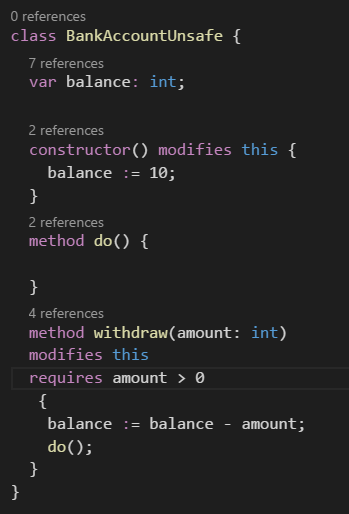
\includegraphics[width=0.5\textwidth]{img/codelensesClosed}
	\caption{Code Lenses used with Dafny}
	\label{fig:agcodelensesclosed}
\end{figure}
When given locations of the references, it is possible to let Visual Studio Code highlight them in the preview window which opens when a codeLens is expanded. Visual Studio Code also groups references according to the file path in the location, so the programmer gets to see a map of all references ordered by containing file to the right of the preview window and can quickly navigate to them.
\paragraph{Why were they chosen to implement}
Since codeLenses can be used to quickly gain a deeper understanding of a code base, it was decided to integrate this feature. Another reason was that it is widespread in different IDEs, so that programmers have become accosted to it. \newline
The first decision to be made was for which elements in the code codeLenses should be displayed. The trade off here is to  provide enough information to work comfortably with the code base and not to clutter the workspace with codeLenses. It was decided to display codeLenses for classes, methods (including constructors) and fields, since they tend to have a wide scope in the code bases \newline
A second consideration was which information should be displayed in a codeLens. When codeLenses are language specific,  references and usages of the element are usually displayed. Since this allows the programmer to gain a deeper understanding of control flow and regions affected by refactoring, it was decided to display this information also for the Dafny plugin. CodeLenses also allow commands to be executed when clicked upon, a logical conclusion is to implement go to reference when a reference in a codeLens is clicked.\newline
\begin{figure}[H]
	\centering
	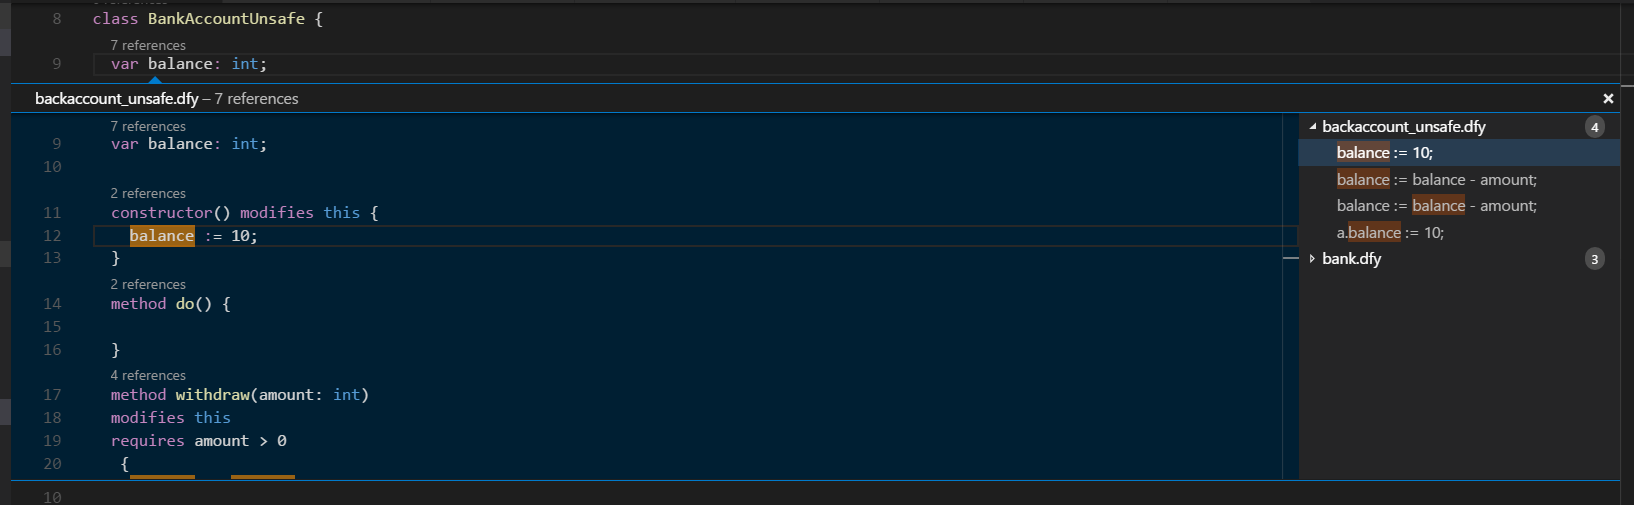
\includegraphics[width=1\textwidth]{img/codelensesExpanded}
	\caption{Expanded CodeLens showing the references to the field balance}
	\label{fig:agcodelensesexpanded}
\end{figure}
\paragraph{What benefits do they entail}
CodeLenses allow to gain understanding of a code base rapidly. Scoping is visible at a glance, making it excellent to find out which regions of code are affected by a refactoring or how many classes rely on another class. By clicking on the references that are listed, one can also navigate the code base with ease, making it easy to follow program flow. \newline
The existing solutions do not yet implement code lenses at all, a feature which is wide spread in other established language integrations. Once a programmer is used to working with code lenses, it usually becomes a feature that is quite heavily used and bring a big improvement in productivity, since relationships do not have to be recorded in a mental model. It stands to reason that this feature brings the biggest improvement in understanding control flow and navigating a code base when compared to other stand alone features, making it an  important part of the plugin.
\subsubsection{Code Completion} \label{agcodecompletion}
\paragraph{What is Code Completion}
Code completion prevents the programmer having to type out every identifier fully. Microsoft calls this feature IntelliSense in its products. Usually, when the programmer starts typing, a little popup appears in which the programmer can choose options that complete the code he is currently writing. The suggestions are usually context aware, because a popup that is cluttered with every identifier in the file currently opened does not bring an improvement in productivity.\newline
\begin{figure}[H]
	\centering
	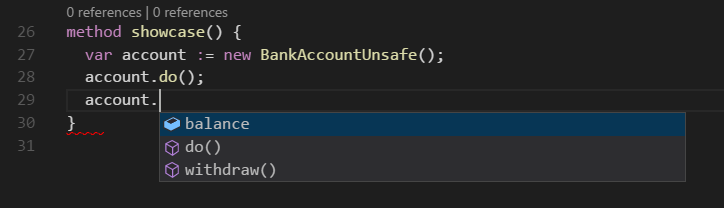
\includegraphics[width=1\textwidth]{img/codeCompletionOverview}
	\caption{Popup with completion options}
	\label{fig:agcodecompletionoverview}
\end{figure}
\paragraph{Why was it chosen to implement}
Since this is arguably one of the most helpful features in IDEs, the implementation thereof was paramount to the completion of this project. Programming in most environments, after the desired algorithm has been thought of, has become equal to the task of writing a few letters and then looking at the completion suggestions of the IDE.  \newline
Almost all modern IDEs offer a way to trigger code completion and this feature is heavily used. The main reason it was chosen to implement is that it brings very big improvements in productivity, freeing the programmer from having to remember all identifiers correctly and having to type them completely.
\paragraph{What benefits does it entail}
As already detailed, the improvement in productivity is huge when using this feature. A programmer that is used to code completion probably never wants to switch back to not using it. Amongst the existing solutions, only the Visual Studio integration offer code completion. This project however tried to go a little further and next to visually distinguishing the types of suggestions (e.g. methods, fields and so on), it also displays existing preconditions of methods in the suggestion popup. \newline
\begin{figure}[H]
	\centering
	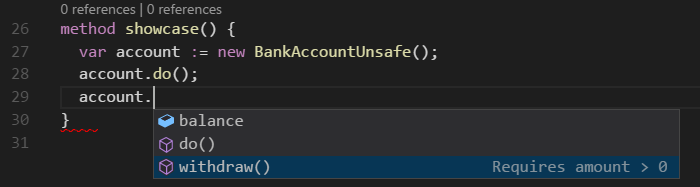
\includegraphics[width=1\textwidth]{img/codeCompletionMethod}
	\caption{Suggestion displaying precondition}
	\label{fig:agcodecompletionmethod}
\end{figure}
This combines a Dafny specific feature with a language agnostic one and lets the programmer know as early as possible under what restrictions he is working under. Being able to provide code completion in this plugin provides programmers with the opportunity to translate their thoughts quickly into code and not having to bother with exact writing.
\subsubsection{Go to Definition} \label{aggotodefinition}
\paragraph{What is Go to Definition}
Another common feature in modern IDEs is go to definition. It enables the programmer to quickly jump to the definition of a code element he is currently working with in order to gain further insight about it. This can usually be done either via a hot key for the current cursor position or an option when opening the context menu via a right click, Visual Studio Code offers both ways.\newline
\begin{figure}[H]
	\centering
	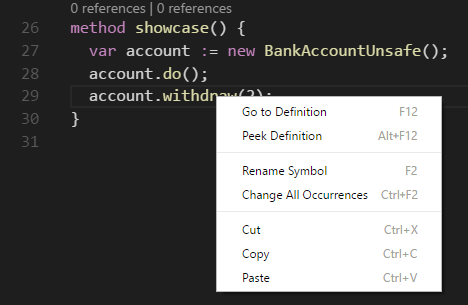
\includegraphics[width=0.5\textwidth]{img/goToDefinition}
	\caption{The Definition Features}
	\label{fig:aggotodefinition}
\end{figure}
Usually this feature offers to either open the code file containing the definition or just to peek at it in a popup. Visual Studio Code supports both these options. If the definition is ambiguous, which often happens when working with interfaces, usually a list of all possible definitions is displayed, because the concrete definition is often impossible to find using static code analysis.
\paragraph{Why was it chosen to implement}
As it is similar to codeLenses, this is a feature which is elemental to all modern IDEs and provides great overview over a project. The implementation of this feature had a high priority in this project. It is also used to navigate in a code base and is actually the reverse application of references in a codeLens, because instead of finding all usages, one jumps from a usage to the definition. \newline
Next to code completion, it is probably the feature most widely implemented in IDEs, so it is important that a Dafny integration does implement it as well, as it provides programmers an idiomatic way of working with a code base.
\paragraph{What benefits does it entail}
Similar to codeLenses, go to definition is a command which can deepen the understanding of a code base profoundly. It is at all times clear where a certain symbol comes from, and one can easily check what it does by jumping to the implementation. It also helps a lot when one has to trace control flow backwards in order to find out where certain data originates from. \newline
The existing solutions do not yet implement go to definition, with the exception of the Visual Studio integration. Being able to quickly navigate to a symbols definition keeps the programmer of having to keep track of all implementations and staying in the current scope of abstraction. If one needs to know more about a symbol, a peek can quickly show the desired information without distracting the train of thought with a new open file in the editor. This makes programmers that use this command usually more efficient and productive.\newline
\begin{figure}[H]
	\centering
	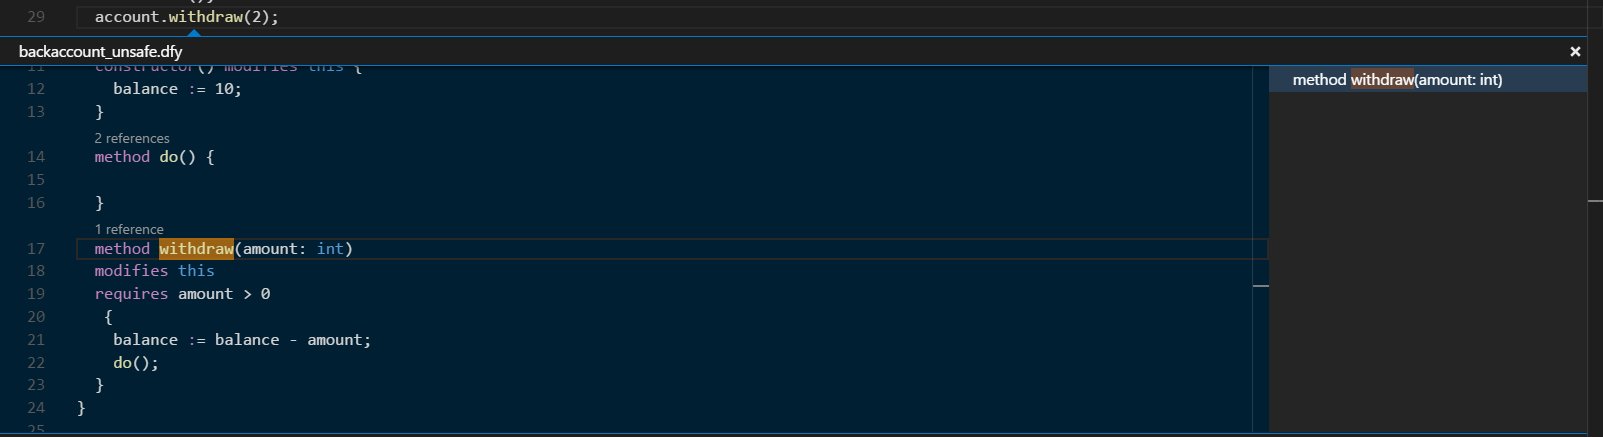
\includegraphics[width=1\textwidth]{img/goToDefinitionPeek}
	\caption{Overlay of peeked definition}
	\label{fig:aggotodefinitionpeek}
\end{figure}
\subsubsection{Rename Element} \label{agrenameelement}
\paragraph{What is Rename Element}
Rename element is a feature essential to refactoring. It is very widespread in IDEs. Visual Studio Code offers built in support for renaming either via a hot key or the context menu. Renaming an element switches all occurrences of an identifier to a new one. This can be a methods, an alias of an object or any other element in a code base. \newline
\begin{figure}[H]
	\centering
	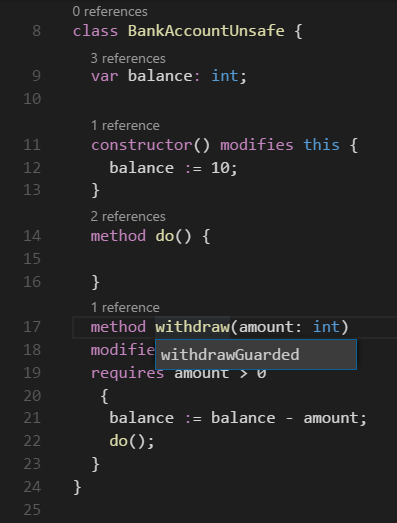
\includegraphics[width=0.5\textwidth]{img/rename}
	\caption{Renaming an element in Visual Studio Code}
	\label{fig:agrename}
\end{figure}
With this feature, one has to be careful when implementing it, since it actually changes the code base and it has to be sure which elements have to be renamed and which do not. There can be several identifiers that are exactly the same but reside in different scopes. When applying the refactoring, only the correct occurrences, which are determined by scope, should be changed while the others must stay untouched. Doing otherwise can change the expressed intent of a program or, if done poorly, can break code.
\paragraph{Why was it chosen to implement}
Because of its importance in refactoring, which is one of the most important tasks when programming, implementing this feature belongs to the core scope of this project. Renaming element allows to quickly make code better readable.\newline
Keeping a code base readable and clean should be one of the biggest concerns when developing a product, a feat which is only accomplished through constant refactoring, a task which is almost impossible to do when renaming of elements is not supported automatically should the code base grow sufficient big enough.
\paragraph{What benefits does it entail}
Renaming of elements allows the programmer to keep the expressed intent of a program in sync with the actual intent when implementations change as they tend to do over time. Normally more time in programming is spent editing or deleting old lines of code than writing new ones. Having automated support in this area does not only make work quicker, but also guarantees for non breaking changes when implemented correctly. When one has to adapt many pieces of code manually, it is almost guaranteed to make a mistake somewhere. \newline
None of the existing solutions support context aware renaming, which is very important if the refactoring should be applied correctly. When writing production quality software, renaming of elements helps to keep the intent clear and make the code base more readable, which is especially important if it has to be maintained for a long lifespan. For these reasons, a programmers that uses this feature often and correctly tends to write more expressive code.
\subsubsection{Syntax Highlighting} \label{agsyntaxhighlighting}
\paragraph{What is Syntax Highlighting}
Syntax highlighting is the feature of displaying different elements in the editor with different colors. Usually there is an IDE idiomatic coloring scheme, so that for instance all language keywords or types are colored the same across different languages, if the IDE supports multiple. \newline
\begin{figure}[H]
	\centering
	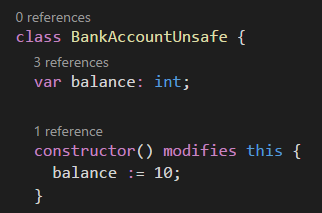
\includegraphics[width=0.5\textwidth]{img/syntaxHighlighting}
	\caption{Syntax Highlighting of Dafny}
	\label{fig:agsyntaxHighlighting}
\end{figure}
Syntax highlighting is usually applied constantly and updates instantly when the programmer types new code. The mechanisms to display the coloring are also very deeply ingrained into the IDE, relaying on a declarative language grammar definition file to do all the coloring. 
\paragraph{Why was it chosen to implement}
Syntax highlighting is definitely the first feature to get working in an IDE, maybe next to run program. Even simple text editors such as Notepad support syntax highlighting for multiple languages, so it is expected of a language integration to come with working highlighting.
\paragraph{What benefits does it entail}
This feature makes code a lot more readable, and a lot more time is spent reading code than writing. It makes the purpose of a symbol clear at first glance thanks to idiomatic coloring. Understanding code becomes much easier when one is guided by colors. Syntax highlighting can also help tracing bugs were the programmer and the compiler do not have the same opinion of a certain syntax, since syntax highlighting reflects the way a compiler interprets a piece of code. \newline
Since this is such a basic feature, all existing solution support this feature, usually relying on the same grammar definition file written for the sublime integration of Dafny \cite{sublime}. This project expanded the implementation a little, also providing syntax highlighting for parameters and generic arguments, something that existing solutions neglect.
\begin{figure}[H]
	\centering
	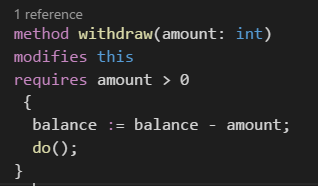
\includegraphics[width=0.5\textwidth]{img/syntaxHighlightingMethod}
	\caption{Syntax Highlighting of parameters}
	\label{fig:agsyntaxHighlightingMethod}
\end{figure}
\subsection{Dafny Specific Features}\label{dffeatures}
This chapter details the language specific features that were implemented during the project. Since Dafny focuses on an elegant way of writing specification constructs, the goal of these features is to aid the programmer writing them. While such constructs have great potential helping to write correct code, most programmers are not yet used to thinking in terms of this methodology. In addition, there are situations which appear often that warrant the writing of similar specification constructs. While important, this work can become tedious. The features detailed in this chapter try to mitigate both these points. \newline
\subsubsection{Counter Examples}
\paragraph{What are Counter Examples}
Dafny's proof pipeline works by trying to find a proof by contradiction. This means, that when a programmer writes a specification construct such as a postcondition, Dafny and its pipeline try to find a situation where the postcondition does not hold. If no violation is found, the proof obligation is satisfied. \newline
If however, a violation is found, that means that the pipeline has found a set of assignments to the variables involved in the context of the postcondition that led to the postcondition being violated. The set of such assignments that lead to a violation is called a counter example. \newline
Counter examples are split up into different states. This means, Dafny includes all assignments to each variable in each state of control flow in a context. This may seem very abstract, but it becomes clear when shown in a simple example. \newline
\begin{figure}[H]
	\centering
	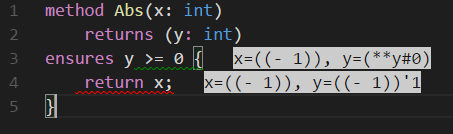
\includegraphics[width=0.8\textwidth]{img/counterModel}
	\caption{Counter Example is shown in Visual Studio Code}
	\label{fig:dfcounterModel}
\end{figure}
When a counter example is generated for a postcondition of a method as seen in \ref{fig:dfcounterModel}, Dafny determines the value of each variable at each point of execution. In the example, there is only one line of code in the method body. This means that the method has two states. The first one is before the line is executed, in this case, only the parameter x is set to a value which will lead the postcondition to be violated. The return value y has not been set yet, so the counter model at this state does not yet hold a value for y. \newline
At the next state of computation, the line in the method body has been evaluated. Dafny's counter model no not only shows the value of x, but also the value of y which can be determined after that line of code has been evaluated. \newline
In summation, a counter model shows the values of all variables involved at all stages of computation that lead to a specification construct being violated. 
\paragraph{Why where they chosen to implement}
To widen the circle of Dafny programmers, it is important to support Dafny specific features in a language integration. Displaying counter example was chosen mainly because of two reasons. The first one is that many programmers are not used to writing specification constructs, so displaying counter examples is a good way to clarify what a specification constructs actually expresses, deepening the understanding of the programmer. \newline
The second consideration is that edge cases are a continuous source of errors. While they may often be forgotten when writing specification constructs, they are most likely the values that Dafny finds to build a counter model with. This quickly leads to the inclusion of edge cases when thinking of error free code, something which is difficult to achieve for IDEs. \newline
A more internal notion on why they were integrated is that, as detailed in \ref{evaluation}, the project failed to deliver a generic approach towards contract generation. Displaying counter examples is a way to partly make up for this missing feature, as it supports the programmer finding correct constructs. 
\paragraph{What benefits do they entail}
Counter examples greatly deepen the understanding of code, as they bring to attention possible situations that the programmer did not think of. When writing complex code, it is nearly impossible to have all possible contexts in mind that it can run and possibly fail in. The displacement of counter examples helps the programmer reasoning on when implementations satisfy specification constructs, which is ultimately the main goal behind the design of Dafny. \newline
They also help writing correct specification constructs, which is not always easy. When constantly being shown counter examples on when a contract is violated, the programmer can refine a contract iteratively until it is no longer violated. This is also the approach that most modern proofing frameworks follow. \newline
\begin{figure}[H]
	\centering
	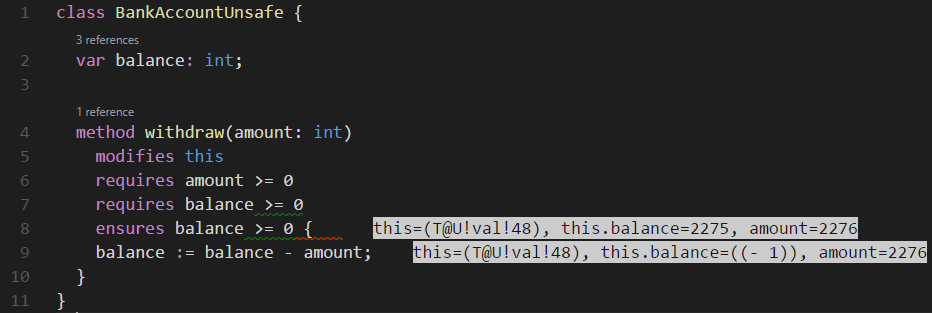
\includegraphics[width=1\textwidth]{img/counterModelBank}
	\caption{Complex Counter Example with multiple specifications}
	\label{fig:dfcounterModelBank}
\end{figure}
As already detailed in the paragraph above, counter examples also often show edge cases that lead to a condition not being satisfied, a very important consideration when programming. These can then easily be taken care of appropriately by the programmer, either by changing the specification construct or the implementation. Without displaying this information, it is very difficult for the programmer to exactly find out how a condition is violated. \newline
This project is the only solution that displays counter examples except for the Visual Studio integration, a feature which is probably the most important Dafny specific aid an IDE can provide. 
\subsubsection{Null Checks}
\paragraph{What are Null Checks}
Null checks are specification constructs that take the form of a precondition that requires an object to be not null. They can be written whenever a new context is opened. Examples are when an object is given as an argument to a method, then the specification is a precondition to the whole method. Another one is when a object is declared, potentially not initialized and used in a later following while block. Then the precondition is written for the while block.\newline
\begin{figure}[H]
	\centering
	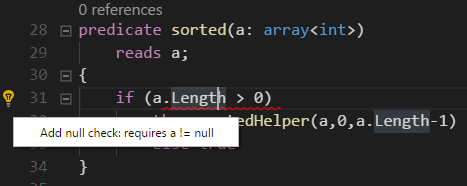
\includegraphics[width=0.7\textwidth]{img/nullCheck}
	\caption{A situation that profits from a Null Check}
	\label{fig:dfnullcheck}
\end{figure}
When a null check is written in form of such a precondition, the following context can safely interact with the object, since it is sure that the object is initialized. 
\paragraph{Why were they chosen to implement}
Programmers very often access members of elements, especially in the methodology of object oriented programming. While it offers a great way to structure a program and to represent reality in a program, it comes with some danger. The most common pitfall usually is the null reference. To help avoid this, Dafny reports potential null references. Since almost any piece of complex code deals with objects, this is a very common occurrence, since for instance every object given as an argument must be checked for null first. \newline
It was therefore decided to offer a mitigation of this important, but tedious work. The insertion of such a precondition shifts the burden of providing valid arguments to the caller of a context, so the implementation can concentrate on providing functionality. While working with Dafny, it was noticed that such a precondition was needed for about every third method, and every other while block, meaning that a lot of work is done for the programmer by supplying this precondition generation.
\newline
Providing this Dafny specific feature was implemented as the first code fix, since a null reference arguably is the most common trivial error when programming in the object oriented methodology. Offering an automated solution to this in an IDE makes Dafny's strengths shine and working with it more enjoyable.
\paragraph{What benefits do they entail}
Current solution do not support the automatic generation of null checks, something which occurs very often when programming. Avoiding null references is important, but tedious work. Providing an automated fix for this enables the programmer to work in a safe context and to concentrate on providing functionality without having to think about checking the context first. \newline
\begin{figure}[H]
	\centering
	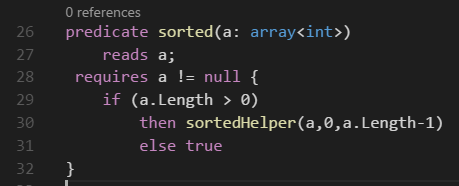
\includegraphics[width=0.7\textwidth]{img/nullCheckApplied}
	\caption{An example of a Null Check}
	\label{fig:dfnullcheckapplied}
\end{figure}
This improves productivity, since it narrows the problems that the programmer has to deal with himself. Providing null checking therefore helps the programmer writing code more quickly and profit from Dafny in an automated way.
\subsubsection{Bound Checks}
\paragraph{What are Bound Checks}
When accessing an array, this is done by providing an expression that is used as an index into that array. Since an array has a fixed length, it is important that the expression resolves to a value inside the array's range. \newline
\begin{figure}[H]
	\centering
	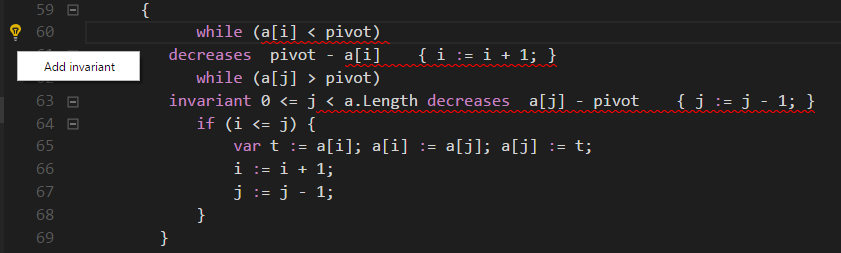
\includegraphics[width=1\textwidth]{img/indexOutRangeDiag}
	\caption{Accessing an array without making sure the index is in bound}
	\label{fig:dfindexOutOfRange}
\end{figure}
Since the definition of an array's range is always the set of integers between zero and the array's length minus one, bound checks can be implemented as two specification constructs that take the form of preconditions belonging to the context in which the array is accessed in. \newline
The first precondition states that the expression used as an index must resolve to a value bigger or equal to zero, the second one that the expression must resolve to a value smaller than the array's length. When these two preconditions hold, it is sure that the array access will succeed and not result into a memory violation. 
\paragraph{Why where they chosen to implement}
Since Dafny has enough knowledge about the array data structure, it issues compilation errors every time an array is accessed without checking for its bounds first. While programming with Dafny, it was observed that this is the case in almost every non trivial example using arrays. Since the array data structure is used quite often in Dafny, it was decided to also help the programmer with this construct, since bound checking is important, but tedious.
\paragraph{What benefits do they entail}
Current solution do not support the automatic generation of bound checking. This task has to be performed very often and is tedious. Relieving the programmer of this repetitive work frees his mind for working on core functionality of a product. \newline
\begin{figure}[H]
	\centering
	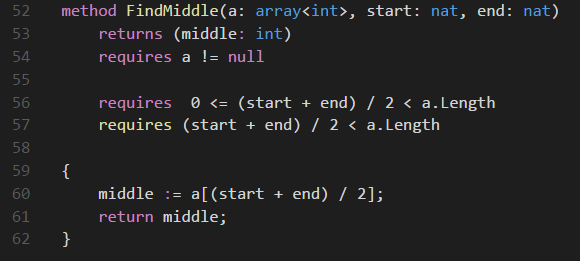
\includegraphics[width=0.8\textwidth]{img/boundCheck}
	\caption{Bound checks were generated}
	\label{fig:dfindexInBound}
\end{figure}
Automatically resolving these checks therefore makes working with Dafny more efficient and is part of making the plugin more usable and supportive.
\subsubsection{Increase / Decrease / Invariant Guards}
\paragraph{What are they}
These constructs that are called guards in this paper help ensuring that an expression complies with certain conditions. This is done by writing specification constructs that ensure this. 
\newline
In case of increase or decrease guards, this is done by either writing an increase or a decrease specification construct, demanding that an expression either increases or decreases. This is often needed to meet loop termination or when using recursion, in both cases Dafny recognizes that an expression should change over time in a certain way and requires constructs detailing this. This makes sure that for instance recursion reaches a termination clause or a loop terminates. \newline
\begin{figure}[H]
	\centering
	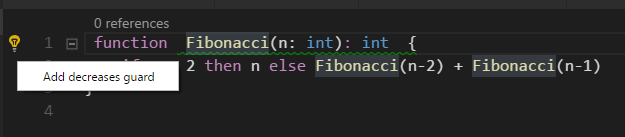
\includegraphics[width=0.7\textwidth]{img/decreaseGuard}
	\caption{Recursion should always decrease an expression}
	\label{fig:dfdecreaseguard}
\end{figure}
In case of invariants, it is done by writing a specification construct called an invariant. When an expression used in an invariant can be dynamic, it specifies to which range of values it can resolve. 
This is for instance needed when an expression used as an index to an array is dynamic inside of a loop. The invariant then makes sure that the expression is always in bound of the array. 
\paragraph{Why were they chosen to implement}
The first two guards are needed to  make sure an expression converges to a certain range of values over time. This is the case when making use of recursion to ensure that the base case is eventually met, or when writing loops that depend on a certain value of an expression for termination. Both examples are very important, because not handling them correctly can result in endless loops or overflow. Dafny already does a good job in generating warnings that tell the programmer that constraints should be enforced for a certain expression. These situations also occur very often, since both recursion and loops are fundamental elements of programming.\newline
Often, an expression must always evaluate into a certain range, this is for instance the case when an expression that is used as an index to an array is not constant within the context of a loop. \newline
Since the above detailed constructs are used often, and the appropriate specification constraints help using them correctly, it was decided to implement an automatic way of generating them. 
\paragraph{What benefits do they entail}
No existing solution offers an automatic way of generating these guards, a tasks which soon was discovered was tedious and time consuming, because it is not always clear at first glance which expressions are subject to constraints. Providing an automatic way of generating them does ensure that the specification constructs are declared correctly, manually inserting them is error prone and demands some reasoning by the programmer.  \newline
\begin{figure}[H]
	\centering
	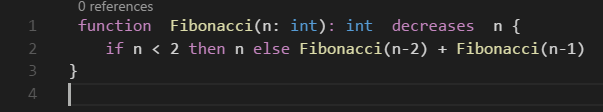
\includegraphics[width=0.7\textwidth]{img/decreaseGuardApplied}
	\caption{Recursion guided by a decrease guard}
	\label{fig:dfdecreaseguardapplied}
\end{figure}
This feature therefore allows the programmer to be more productive and concentrate on key areas of concern.
\subsubsection{Flow Graphs}
\paragraph{What are they}
A existing feature in Boogie is to translate boogie programs into a flow graph. It does not only show the flow of the program itself but also includes all pre- and postconditions. Below is an example of a flowgraph, taken from the partition method of a quicksort algorithm.\newline  
\begin{figure}[H]
	\centering
	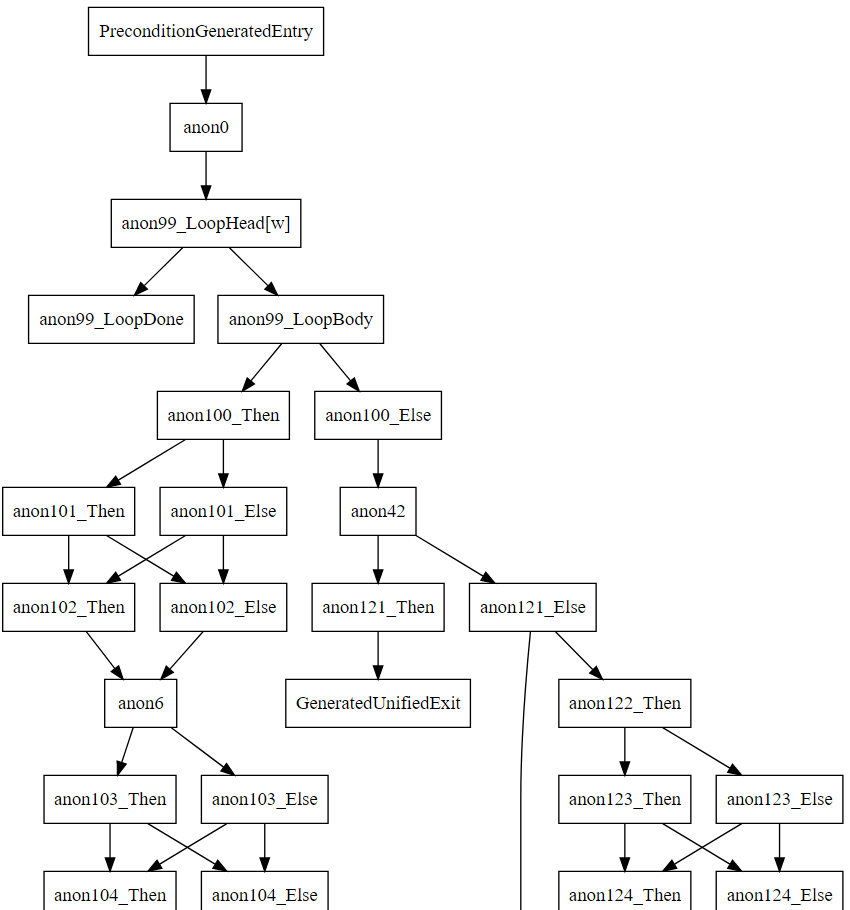
\includegraphics[width=0.9\textwidth]{img/flowgraph}
	\caption{Flow Graph of the partition method}
	\label{fig:flowgraph}
\end{figure}
\paragraph{Why were they chosen to implement}
Because this feature existed already in Boogie, and the goal was to support as many features from the Dafny pipeline as possible, it was decided that this feature could be easily and nicely implemented. 
\paragraph{What benefits do they entail}
Developers can directly see the flow of the program they are working on in Visual Studio Code. Otherwise, they would need to manually save the graph to a file, upload or convert the file to finally view it. This all is done in the background to provide a nice user experience.

\section{Possible points for Extension} \label{extensions}
This chapter details what further work could be done on the plugin by subsequent projects.

\subsection{Support for other IDEs} \label{ides}
Since the plugin is structured as a language server, it should theoretically be possible to integrate it into any IDE which implements the language server protocol without any problems. In reality, some customization is often needed and some popular IDEs also do not fully implement the protocol yet. This chapter details which IDEs were looked at as possible hosts for the plugin and what would have to be done for a complete integration.
\subsubsection{Eclipse integration}
The eclipse project \href{https://projects.eclipse.org/projects/technology.lsp4e}{LSP4E} aims to integrate existing language servers into the Eclipse IDE in an easy way. 
\newline
"It includes some APIs to turn language server protocol elements into Eclipse IDE concepts and a generic integration allowing to easily plug any language server to an Eclipse IDE instance without need to write Java code, either via a plugin associating a new language server, or by letting users manually bind language servers to their IDE." \cite{lsp4e}
It is built on top of \href{https://github.com/eclipse/lsp4j}{LSP4J}, a Java implementation of the language server protocol. 
\newline
Integrating the Visual Studio Code Dafny language server into Eclipse could become possible in the future. Right know there is no way to interact on the client side. One only can specify a language server based on a program (NodeJS) and arguments (extension.js) which is executed and used for querying information. One cannot add any behavior to Eclipse itself, which would be necessary for certain features. Also, the sendRequest protocol specification is not implemented yet (Commit: 1615e07), which is important for starting the DafnyServer correctly. 
The better way would be to program a new Eclipse plugin, based on LSP4J, which then would also allow to customize the status bar, run scripts and show progress information. 
\subsubsection{Emacs integration}
Emacs \cite{GNU} is a versatile IDE which enjoys great popularity especially in the open source community. Written in LISP, Emacs traditionally supported language integration via so called modes, which are demons that run in the background. This is already a similar architecture as used in a language server integration. \newline
Work on integrating language servers into Emacs has already be done. The project emacs-lsp \cite{emacsLsp} aims to provide the connection between Emacs and language server. The project itself is structured as a classical Emacs demon and allows interactions with a language server. There already exist some integrable language servers in languages such as Java or Haskell. The integration of emacs-lsp and existing language servers seems to be pretty trivial, an example can be seen in \cite{javaEmacs} using Java. \newline
Since the language server allows custom messages to be defined as detailed in the implementation documentation, the Dafny plugin defines some of them. One set of custom messages is necessary, since the plugin allows for downloading the Dafny compiler automatically. The communication in regard to this feature must be extended to the IDE, so that the user is aware of this feature. Additional custom components are the state of the file so that the programmer sees if it is verified or not, or the displaying of counter examples for proofs.\newline
These features were deemed very useful in this project, such that they should be a part of every IDE integration. This means that a little wrapper would have to be written on the client side of the language server, which understands the custom messages and can relay this information to the IDE itself. The work that has to be done is trivial, since it simply means to pass information on and display them accordingly. \newline
It was decided that gaining a working knowledge of LISP and Emacs in order to write such a wrapper was not in the scope of this project. For a programmer familiar with Emacs and LISP this task should take no more than a week. The custom messages that need to be implemented can be found in the implementation documentation. It can be argued that this extension should be one of the first ones to be tackled by later work, as one can gain a considerably larger user base without having to invest too much work. 
\subsubsection{Monaco integration}
Monaco\cite{monaco} is the code editor that powers Visual Studio Code. It is also possible to use Monaco as a standalone editor in the browser. It would be interesting to integrate Dafny directly into Monaco, since there are not many simpler setups imaginable as opening a browser window. It was therefore decided to look into a possible integration of the plugin during the course of this project. \newline
It soon became apparent that the project does not seem very active, as the latest commit was two months old at the time of this writing. The documentation for developers is also very sparse. There was hope that an integration would be trivial, since the plugin is structured as a language server. However, Monaco does not implement the language server protocol. In the documentation, it can even be read that "Extensions written for Visual Studio Code will not run in Monaco"\cite{monaco}, without any further explanation given. \newline
However, integrating a new language into Monaco is possible, as can be seen in an example for Typescript in  \cite{monacoType}. However, the setup is different than a language server integration or a Visual Studio Code plugin. It is questionable how much code could be shared. While the idea of running Dafny in an editor in the browser is interesting, the work that would have to be done in order to achieve this was deemed to be outside of the scope of this project. In addition, if further work aims to implement this integration, an evaluation on how active the work on Monaco is should be done first, given the apparent standstill in the project at the time of this writing.
\subsection{New Features} \label{featureExtensions}
This section details some interesting ideas that were gathered during development of the plugin, but were sadly out of scope of this project. It is thought as a starting point for developers that want to extend this plugin. 
\subsubsection{Debugger}
Integrating a debugger into the plugin would be great, since this is a feature that is very often used and very helpful when searching for bugs. An existing solution already support this feature, namely the Visual Studio integration \cite{visualstudiodafny} of Dafny. This already works very well and can be used as a guideline when developing an own integration. It is also a feature that programmers have become used to in all modern IDEs so it should be part of any language integration. \newline
Sadly it is also quite a difficult task since the interaction between an IDE, an executable and a debugger is complex. While the Visual Studio integration is open source, it is written in C\# and can therefore interface directly with the Dafny pipeline, which is heavily done in that integration. It would take quite some work to abstract this direct interaction into a clean API that extends the existing API of the Dafny pipeline. Using this API, a language server could provide an own implementation of a debugger.\newline
Designing this complex component was well out of scope for this project. It is estimated that, depending on the preexisting knowledge, this would be an endeavor of about two to four weeks time and probably would have to rely on at least some help by the Dafny development team. While this task is difficult, the result would be having an important feature that all users of modern IDEs anticipate in a language integration. It therefor should be a primary consideration when deciding on how to extend this project. 
\subsubsection{Widening Scope}
While many features have been implemented during the course of this project, the scope of their application was often narrowed as to provide a pragmatic approach to the problems regarding the scope of the project. For example, the rename element refactoring only works on members of classes, but not on parameters of methods. \newline
The exact scope of all features can be found in the API documentation of this project. While the extension of scope of existing features might seem tedious and not very interesting, it can introduce subtle problems that have to be dealt with with great care. It also is benefical to the users, as they can apply features in much wider contexts. 
\subsubsection{Contract Generation}
While contract generation has been implemented for some often occurring situations as detailed in \ref{dffeatures}, there is still a big potential for improvement in this area. Since a generic approach to contract generation has been deemed to be unfeasible, the next best way is to offer help in writing specification constructs in specific situations.\newline
When deciding to do work in this area, it is important to first analyze which situations appear often in a typical Dafny program. While this task it is difficult in itself, since it requires some expertise in Dafny, it is important because otherwise features may be implemented that do not get used in every day scenarios. \newline
When such situations have been identified, the specification construct generation must absolutely be correct. Since this is a feature that changes existing code, it is better to not provide any help when there is ambiguity regarding the correct solution. However, when done correctly, this is a feature from which programmers can greatly benefit, since it enhances productivity by eliminating the need to do complicated reasoning. It also introduces capabilities of Dafny to programmers that are not yet proficient in their usage of the language.



\section{Conclusion}
The section concludes this paper by first comparing the reached goals with the stand of the existing solutions. In the end, an evaluation of the project is detailed. 

\subsection{Reached Goals}

\subsubsection{Platform Indepence}
\subsubsection{Setup}
\subsubsection{Usability}
\subsubsection{IDE Independence}
\subsubsection{Feature Richness}
\subsection{Evaluation}\label{evaluation}
Following the comparison made in \ref{golrech}, it can safely be said that product developed during this project is at least en pair with most existing solutions. An automated setup of the entire environment which resolves dependencies on all major platforms guarantees that new users can make their first steps with Dafny without having to spend time to get things running. This is an important first stepping stone in making Dafny accessible for a wide user base. \newline
After having gotten Dafny to run on an environment, the next concern is to offer a productive, efficient and enjoyable programming experience. This keeps programmers using Dafny interested and keen on further using it. Having implemented many common IDE features as well as some Dafny specific functionality lets programmers apply work flows they have established with other languages as well as discovering the big benefits regarding functional correctness Dafny can offer. \newline
Structuring the plugin as a language server decouples it from any particular IDE, although this project relied on Visual Studio Code as a reference IDE. This decoupling leads to the possibility to integrate Dafny into many other IDEs without having to duplicate any logic. This further lays the groundwork to support a wide user base as a programmer would not have to switch the IDE he has come used to for another one. \newline
Offering generic contract generation sadly was established to be not feasible to implement in the scope of this project. During this research it was found that this problem probably also is unsolvable due to the proof pipeline that Dafny uses. Instead of offering generic generation, often arising situations were identified and aids provided for them.\newline
It was a major concern for this project to not just develop a proof of concept, but a production ready release of the plugin. Through the application of continuous integration feedback from users could be integrated early on. The plugin has been already downloaded over 300 times from all over the world at the time of this writing. It was also used in a course concentrating on software engineering at a school for higher education to get students familiar with contract based reasoning. During this, the plugin was used by about 60 students, underlining the robustness and platform independence of the solution. The minor changes that had to be made to the Dafny pipeline itself during this project have been accepted by Microsoft and are integrated into the official version of the pipeline. \newline
The open source nature of this project encourages people to participate in enriching the plugin, as well as integrating it in additional IDEs. Close detail has been paid on keeping the documentation as well as the code quality at a high standard, so contributing should be possible without having to invest too much time to get started. It stands to hope that providing the plugin in the state it is at the end of this project is a big stepping stone in widening the user base that can profit from using Dafny. 

\newpage
\appendix
\pagenumbering{Roman}
\section{Project management}
\subsection{Projectplan}
\begin{figure}[H]
	\centering
	\includegraphics[width=1.2\textwidth]{img/projectplan}
	\caption{Projectplan}
	\label{fig:Projectplan}
\end{figure}
\subsection{Milestones}
\rowcolors{1}{gray!25}{white}
\begin{longtable}[H]
	{l| l | p {0.7\textwidth}}
	\textbf{Nr} & \textbf{Title} & \textbf{Description} \\ 
	\hline\hline
	
	M1 & First prototype & Plugin is working on all operation systems, simple verification is in place and errors are reported, basic syntax highlighting \\ 
	
	M2 & Improved prototype & Automatic downloading of dependencies and installation of Dafny and configure of environment variables \\ 
	
	M3 & Contract generation & First automatic contract generation, customizable with DSL \\ 
	
	M4 & Autocompletion & Autocompletion for identifiers \\ 
	
	M5 & Release 1.0 & Everything implemented and tested. Ready to be published \\ 		
	\caption{Milestone}
	\label{tab:Milestone}
\end{longtable}
\subsection{Risk management}
\begin{landscape}
	\rowcolors{2}{gray!25}{white}
	\begin{longtable}[H]
		{l|p{0.22\textwidth}| p{0.22\textwidth} | p{0.1\textwidth} | p{0.1\textwidth} | p{0.25\textwidth} | p{0.25\textwidth}}
		
		\textbf{Nr} & \textbf{Title} & \textbf{Description} & 
		\textbf{Max Harm [h]} & \textbf{Proba- bility} & \textbf{Prevention} &  
		\textbf{Behaviour at entry}\\ \hline
		
		R1 & Underestimation of workload & One or more team members can't finish a feature in time or loses to much time on a minor feature & 120 & 25\% & Weekly scrum meetings with feedback about the current work progress. Estimate workload together. Include time reserve & Help each other, if one is struggling. Feature reduction as last resort. \\ 
		
		R2 & Workflow is not working & Toolchain is not working as planed. The used components aren't ideal for the problem & 30 & 15\% & Use experience to get a good setup and test it alot in the beginning & Redefine toolchain or change single tool \\ 
		
		R3 & Communication problems & Team is not working together and each member is developing individually. Creation of incompatible interfaces. Talking with the industrial partner isn't possible as expected, due to time difference or not enough time & 70 & 20\% & Weekly scrum meetings and agreements. Already worked in other projects as a team before & Increase written documentation and working closer together. Having a fixed meeting with the industrial partner \\ 
		
		R4 & Lack of knowledge & Team has to little knowledge about Dafny, VSCode and the development of a VSCode Plugin & 80 & 10\% & Already experience with typescript for plugin development, as preparatory work informed about Dafny & Find necessary knowledge online, get help from Microsoft Research \\ 
		
		R5 & Data loss or manipulation & Data loss because of a server crash or open permissions to access and modify data & 20 & 3\% & Regularly backups and restrictive permissions to change files & Use backup to restore data. Extend safety measures \\ 
		
		R6 & Failure developer machine & One of the developer machines isn't working anymore. & 10 & 1\% & Limited, regularly commits and backups. & Switch temporary to the school computer and install the necessary tools. \\
		
		R7 & Implementing the DSL is too complicated or too difficult to use & The DSL would be needed to suggest possible contracts or to customize the best practices. & 100 & 30\% & This core feature has to be researched carefully so that it really fits our needs and that other developers can really use the plugin. & Read about DSL, talking to people which have already worked with it. \\
		
		R8 & Supporting all features on the different environments is not possible & Due to that Windows, OSX and Linux are quite different, it could be that some features aren't possible to implement on a platform or causes a big overhead to get it running & 10 & 25\% & Using as much of the standard API as possible. Implement specific features platform dependant. & Disable a certain feature on a platform or look for a workaround. \\	
		
		R9 & Automatic installer of Dafny is not possible & Maybe because of security restrictions, it could be possible that you can't download and install additional software and set environment variables. & 35 & 20\% & Test if downloading of software can done inside VS Code. & Automatic installer can't be done inside the plugin. Switch to a different strategy and implement an automatic installer over a additional executable, which could also install the plugin in vscode. \\
		
		\caption{Risk management}
		\label{tab:Risk management}
	\end{longtable}
\end{landscape}

\subsection{Risk Matrix}
\begin{figure}[H]
	\centering
	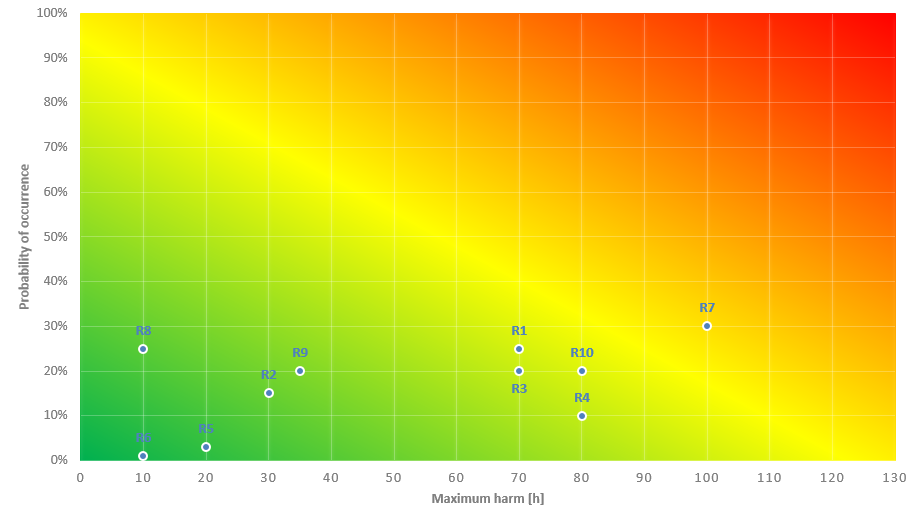
\includegraphics[width=1\textwidth]{img/riskmatrix}
	\caption{Risk Matrix}
	\label{fig:Risk Maxtrix}
\end{figure}
\section{Use Cases}
\subsection{Use Case Diagram}
\begin{figure}[h]
	\centering
	\includegraphics[width=1\linewidth, height=5in]{"./img/UseCase"}
	\caption{Use Case Diagram}
	\label{fig:usecase-diagram}
\end{figure}
\subsection{Actors and Stakeholder}
\begin{itemize}
	\item Programmers
	\item Microsoft
\end{itemize}
\subsection{Descriptions (brief)}
\subsubsection{UC1: Windows Installation}
A programmer can install the Dafny Plugin on his .Net environment running on Windows 10.
\subsubsection{UC2: Linux Installation}
A programmer can install the Dafny Plugin on his mono environment running on a common Linux distribution such as Ubuntu 16.04.
\subsubsection{UC3: OSX Installation}
A programmer can install the Dafny Plugin on his mono environment running on OSX ??? (VERSION).
\subsubsection{UC4: Easy installation of Dafny plugin}
A programmer can simply install the Dafny plugin by running an automatic installer which sets all path variables and makes additional needed environment adjustments.
\subsubsection{UC5: Syntax Highlighting}
The system automatically does syntax highlighting while the user writes a Dafny (dfy.) file.
\subsubsection{UC6: Reporting of Dafny best practices violations}
The plugin can be configured with a simple DSL config file which describes common best practices for Dafny. The plugin reports violations of these rules via the standard Visual Studio Code notification mechanisms.
\subsubsection{UC7: Automatic generation of contracts}
The plugin can be configured with a simple DSL-File to recognize certain semantics, which could benefit from the setting of Pre- and Postconditions. The plugin offers to add these in form of a refactoring via the common Visual Studio Code mechanisms.
\subsubsection{UC8: Autocompletion for identifiers}
The plugin offers autocompletion of Dafny code while the user types via the standard Visual Studio Code mechanisms.
\subsection{Descriptions (fully dressed)}
\subsubsection{UC1: Windows Installation}
\rowcolors{1}{gray!25}{white}
\begin{longtable}{l | p{0.7\textwidth} }
	Description & A programmer can install the Dafny Plugin on his .Net environment running on Windows 10.\\ \hline
	Primary Actor & Programmer\\ \hline
	Trigger & Programmer wants to programm Dafny in Visual Studio Code.\\ \hline
	Stakeholder and Interests & 
	\begin{itemize}
		\item Programmer: Wants stable support from the IDE while developing Code.
		\item Microsoft: Wants a stable Dafny integration to fulfill the needs of its clients.
	\end{itemize} \\ \hline
	Preconditions & 
 \begin{itemize}
		\item Windows 10 Environment with a modern version of the .Net Framework installed.
	\end{itemize} \\ \hline
	Postconditions & 
	\begin{itemize}
		\item The plugin works without problems, the programmer can start writing code.
	\end{itemize} \\ \hline
	Main Success Scenario & 1. Programmer downloads the plugin. \newline
	2. During an automated installation routine, the plugin installs itself and all needed environmental changes are made. (UC4) \newline
	3. Visual Studio code is updated to use the plugin, a success message is shown\\ \hline
	Extensions & 
	2a. The installer notices that some dependencies are missing. \newline 
	- It notifies the programmer accordingly.\\ \hline
	Special Requirements & None\\ \hline
	Frequency of Occurence & Usually once per working environment\\ \hline
	Open Issues & None \\ \hline
	\caption{UC1}
\end{longtable}
\subsubsection{UC2: Linux Installation}
\begin{longtable}{l | p{0.7\textwidth} }
	Description & A programmer can install the Dafny Plugin on his mono environment running on a common Linux distribution such as Ubuntu 16.04.\\ \hline
	Primary Actor & Programmer\\ \hline
	Trigger & Programmer wants to programm Dafny in Visual Studio Code.\\ \hline
	Stakeholder and Interests & 
	\begin{itemize}
		\item Programmer: Wants stable support from the IDE while developing Code.
		\item Microsoft: Wants a stable Dafny integration to fulfill the needs of its clients.
	\end{itemize} \\ \hline
	Preconditions & 
	\begin{itemize}
		\item A modern common Linux distribution such Ubuntu 16.04 or Fedora with the mono framework installed.
	\end{itemize} \\ \hline
	Postconditions &
	\begin{itemize}
		\item The plugin works without problems, the programmer can start writing code.
	\end{itemize} \\ \hline
	Main Success Scenario &
	1. Programmer downloads the plugin. \newline
	2. During an automated installation routine, the plugin installs itself and all needed environmental changes are made. (UC4) \newline
	3. Visual Studio code is updated to use the plugin, a success message is shown\\ \hline
	Extensions &
	2a. The installer notices that some dependencies are missing. \newline
	- It notifies the programmer accordingly.\\ \hline
	Special Requirements & None\\ \hline
	Frequency of Occurence & Usually once per working environment\\ \hline
	Open Issues & None \\ \hline
	\caption{UC2}
\end{longtable}

\subsubsection{UC3: OSX Installation}
\begin{longtable}{l | p{0.7\textwidth} }
	Description & A programmer can install the Dafny Plugin on his mono environment running on OSX.\\ \hline
	Primary Actor & Programmer\\ \hline
	Trigger & Programmer wants to programm Dafny in Visual Studio Code.\\ \hline
	Stakeholder and Interests & 
	\begin{itemize}
		\item Programmer: Wants stable support from the IDE while developing Code.
		\item Microsoft: Wants a stable Dafny integration to fulfill the needs of its clients.
	\end{itemize} \\ \hline
	Preconditions &
	\begin{itemize}
		\item A modern version of the OSX OS installed such as canberra with the mono framework installed.
	\end{itemize} \\ \hline
	Postconditions &
	\begin{itemize}
		\item The plugin works without problems, the programmer can start writing code.
	\end{itemize} \\ \hline
	Main Success Scenario & 1. Programmer downloads the plugin. \newline
	2. During an automated installation routine, the plugin installs itself and all needed environmental changes are made. (UC4) \newline
	3. Visual Studio code is updated to use the plugin, a success message is shown\\ \hline
	Extensions & 
	2a. The installer notices that some dependencies are missing. \newline 
	- It notifies the programmer accordingly.\\ \hline
	Special Requirements & None\\ \hline
	Frequency of Occurence & Usually once per working environment\\ \hline
	Open Issues & None \\ \hline
	\caption{UC3}
\end{longtable}

\subsubsection{UC4: Easy installation of Dafny plugin}
\begin{longtable}{l | p{0.7\textwidth} }
	Description & A programmer can simply install the Dafny plugin by running an automatic installer which sets all path variables and makes additional needed environment adjustments.\\ \hline
	Primary Actor & Programmer\\ \hline
	Trigger & Programmer wants install the Dafny plugin to visual studio code.\\ \hline
	Stakeholder and Interests & Programmer: Wants an easy, automated installation of the plugin. \newline Microsoft: Wants a stable Dafny integration to fulfill the needs of its clients.\\ \hline
	Preconditions &\begin{itemize}
		\item Depending on the environment, the preconditions of UC1, UC2 or UC3 are satisfied.
		\item Visual Studio Code is installed.
		\item The programmer has admin priviledges in his environment.
	\end{itemize}\\ \hline
	Postconditions & 
	\begin{itemize}
		\item The plugin works without problems, the programmer can start writing code.
	\end{itemize} \\ \hline
	Main Success Scenario & 
	1. Programmer downloads the plugin via the Visual Studio Code plugin store. \newline
	2. The plugin determines which platform it is run on, and sets either the path to the .Net framework or the mono framework. \newline
	3. The plugin downloads the Dafny and sets the path to the Dafny server binary. \newline
	4. The plugin then installs itself via the standard Visual Studion Code plugin mechanisms. \newline
	5. The plugin prompts a success message and the programmer is ready to code in Dafny.\\ \hline
	Extensions & 
	2a. The installer can't find, depending on the enviroment, either the mono or the .Net framework in the standard locations. \newline 
	- It prompts the user to enter the location and does so until the framework is found. \\ \hline
	Special Requirements & None\\ \hline
	Frequency of Occurence & Usually once per working environment\\ \hline
	Open Issues & None \\ \hline
	\caption{UC4}
\end{longtable}

\subsubsection{UC5: Syntax Highlighting}
\begin{longtable}{l | p{0.7\textwidth} }
	Description & The system automatically does syntax highlighting while the user writes a Dafny (dfy.) file.\\ \hline
	Primary Actor & Programmer\\ \hline
	Trigger & Programmer writes Dafny code in Visual Studio Code.\\ \hline
	Stakeholder and Interests & Programmer: Wants enhanced readability for the source files he's working on. \newline Microsoft: Wants a state of the art IDE integration of Dafny.\\ \hline
	Preconditions &
	\begin{itemize}
		\item Visual Studio Code with the Dafny plugin installed is running.
		\item Dafny code is being written in a .dfy file.
	\end{itemize}\\ \hline
	Postconditions &
	\begin{itemize}
		\item The source code is highlighted in different colors according to common standards in general and the Visiual Studio Code guidelines specifically.
	\end{itemize}\\ \hline
	Main Success Scenario & 
	1. Programmer types code into a .dfy file. \newline
	2. The plugin detects the changes and applies syntax highighlighting through the standard Visual Studio Code mechanisms.\\ \hline
	Extensions & 
	2a. The newly written code causes a compilation error and cannot be interpreted. \newline 
	- The previous syntax highlighting stays in place, the errors are highlighted according to common practices with compilation errors in Visual Studio Code. \\ \hline
	Special Requirements & None\\ \hline
	Frequency of Occurence & Very often, after every key up event.\\ \hline
	Open Issues & None \\ \hline
	\caption{UC5}
\end{longtable}

\subsubsection{UC6: Reporting of Dafny best practices violations}
\begin{longtable}{l | p{0.7\textwidth} }
	Description & The plugin can be configured with a simple DSL config file which describes common best practices for Dafny. The Plugin reports violations of these rules via the standard Visual Studio Code notification mechanisms.\\ \hline
	Primary Actor & Programmer\\ \hline
	Trigger & Programmer writes Dafny code in Visual Studio Code.\\ \hline
	Stakeholder and Interests & Programmer: Wants to write the cleanest code possible using common Dafny idioms. \newline Microsoft: Wants to support programmers getting the most out of Dafny.\\ \hline
	Preconditions &
	\begin{itemize}
		\item Visual Studio Code with the Dafny plugin installed is running.
		\item Dafny code is being written in a .dfy file.
	\end{itemize}\\ \hline
	Postconditions &
	\begin{itemize}
		\item Violations of common best practices for Dafny are reported through the standard Visual Studio Code mechanisms.
	\end{itemize}\\ \hline
	Main Success Scenario & 
	1. The plugin is installed preconfigured with a collection of common best practives for Dafny, which is done through a DSL file. \newline
	2. Programmer types code into a .dfy file. \newline 
	3. The plugin continuously checks for violations of the rules. \newline 
	4. If a violation is detected, it is reported through the standard mechanisms of Visual Studio Code.\\ \hline
	Extensions & 
	1a. The predefined rules are not sufficient for the programmer. \newline 
	- The programmer can updated the configuration file himself to include his own or his company's coding guidelines. \\ \hline
	Special Requirements & None\\ \hline
	Frequency of Occurence & Very often, after new valid syntax was written.\\ \hline
	Open Issues & None \\ \hline
	\caption{UC6}
\end{longtable}

\subsubsection{UC7: Automatic generation of contracts}
\begin{longtable}{l | p{0.7\textwidth} }
	Description & The plugin can be configured with a simple DSL-File to recognize certain semantics, which could benefit from the setting of Pre- and Postconditions. The plugin offers to add these in form of a refactoring via the common Visual Studio Code mechanisms.\\ \hline
	Primary Actor & Programmer\\ \hline
	Trigger & Programmer writes Dafny code in Visual Studio Code.\\ \hline
	Stakeholder and Interests & Programmer: Wants to write the correctest code possible making use of Dafny's specification constructs. \newline Microsoft: Wants to support programmers getting the most out of Dafny.\\ \hline
	Preconditions &
	\begin{itemize}
		\item Visual Studio Code with the Dafny plugin installed is running.
		\item Dafny code is being written in a .dfy file.
	\end{itemize}\\ \hline
	Postconditions &
	\begin{itemize}
		\item Specification constructs suitable for the context were added as refactorings.
	\end{itemize}\\ \hline
	Main Success Scenario & 
	1. The plugin is installed preconfigured with a collection of common semantics for Dafny and their corresponding specification constraints, which is done through a DSL file. \newline
	2. Programmer types code into a .dfy file. \newline 
	3. The plugin continuously checks for semantics that could benefit form the setting of specification constraints. \newline 
	4. If such a semantic is detected, it is reported through the standard mechanisms of Visual Studio Code, with a refactoring offered to add the constraints. \newline
	5. The programmer invokes the refactorings and the necessary code is added.\\ \hline
	Extensions & 
	1a. The predefined semantics and refactorings are not sufficient for the programmer. \newline 
	- The programmer can updated the configuration file himself to include support for his own or his company's  common code semantics. \\ \hline
	Special Requirements & None\\ \hline
	Frequency of Occurence & Very often, after new valid syntax was written.\\ \hline
	Open Issues & None \\ \hline
	\caption{UC7}
\end{longtable}

\subsubsection{UC8: Autocompletion for identifiers}
\begin{longtable}{l | p{0.7\textwidth} }
	Description & The plugin offers autocompletion of Dafny code while the user types via the standard Visual Studio Code mechanisms.\\ \hline
	Primary Actor & Programmer\\ \hline
	Trigger & Programmer writes Dafny code in Visual Studio Code.\\ \hline
	Stakeholder and Interests & Programmer: Wants enhanced productivity while writing Dafny code. \newline Microsoft: Wants a state of the art IDE integration of Dafny.\\ \hline
	Preconditions &
	\begin{itemize}
		\item Visual Studio Code with the Dafny plugin installed is running.
		\item Dafny code is being written in a .dfy file.
	\end{itemize}\\ \hline
	Postconditions &
	\begin{itemize}
		\item An identifier was autocompleted.
	\end{itemize}\\ \hline
	Main Success Scenario & 
	1. Programmer types code into a .dfy file. \newline
	2. The plugin detects the changes and searches for the beginning of known identifiers. \newline
	3. If such a beginning is found, completion if offered through the standard mechanisms of Visual Studio Code.\\ \hline
	Extensions & 
	None. \\ \hline
	Special Requirements & None\\ \hline
	Frequency of Occurence & Very often, after every key up event.\\ \hline
	Open Issues & None \\ \hline
	\caption{UC8}
\end{longtable}
%\section{Personal Summaries}

\subsection{Personal Summary Markus Schaden}
At the beginning of this project, I was exited but also a little bit nervous about the following weeks. I already did some IDE integration during the term thesis, but the required core features were distinct from the bachelor thesis. Not only did we have to implement a complete new language into Visual Studio Code, but Dafny also is specification construct driven, a programming language type which I rarely worked with. \newline
After the first weeks, we did some good progress, although our project plan was quite ambitious. Especially the preparation looking at the tutorials helped. Unfortunately there was no documentation about the source code. Thereby the only chance to develop new features, was to debug through the code. This helped to gain a understanding about how the verification is working under the hood. The first highlight was, when the export of the symbol table worked for the first time and after a lot of trial and error the project finally successfully compiled.  \newline
During the next couple of weeks my understanding of the Dafny pipeline got better and better. It also became much clearer how the three components are working together. Especially when I started implementing the counter examples, I already knew where to start in order to implement this important feature.  \newline
Due to various other project were I worked with Rafael, I knew that the collaboration with him will be pleasant. During tedious work or if one of us was struggling, it was helpful to work together to overcome problems. Also the discussions and code reviews helped to finish this project in time and with success.   \newline
Farhad Mehta looked after us in a pleasant way. We had the freedom to make decisions and develop, but we also could rely on him if we had problems or needed a third opinion about a topic. Especially he was very helpful in making us understand the proof theory much better. Without this, implementing the counter examples was not possible and we would still be struggling with contract generation, which is not possible with our current knowledge. Also his extensive feedbacks helped to optimize the report and to make the plugin better.  \newline
I really liked to work on this bachelor thesis and am happy with the result. Next to that I learned a lot in various directions, it was a very exiting project. Since we already released the plugin after some weeks, it is a good feeling to know that it is used around the globe. Due to the open source license and the detailed documentation, it would be very nice if some people would start to extend the functionality of the plugin.   \newline
\clearpage
\subsection{Personal Summary Rafael Krucker}
The work on this project has been a very existing and informative experience. While having previously worked on IDE plugins, it was something entirely different integrating an entire language, especially one that is specification constructs driven, something which I also was not very experienced in. \newline
Our project plan was pretty ambitious, while having no experience in proof theory we wanted to integrate a generic way to propose specification. While this task would be very interesting, it soon became apparent that it was not feasible with our knowledge in proof theory and the project scope. Additionally, existing literature suggests that this problem is almost unsolvable hard anyway when working with the kind of proof engine that the Dafny pipeline uses. However, it was very interesting to gain a working knowledge in this area. \newline
After the above mentioned problem was discovered, we reduced our ambitions to provide solutions to concrete problems, which we discovered emerge quite often during programming. It was interesting to isolate situations that programmers could be helped with while it still had to be feasible to provide this help. At the end of this project, I am quite content with the Dafny specific features that we were able to implement, ranging from automatic null checking up unto providing decrease guards. This relieves the programmer of much tedious, but important work. \newline
Farhad Mehta was always quick to break down problems to an understandable point of abstraction when we got stuck somewhere and also provided many important suggestions and ideas throughout our work. This made us progress smoothly while still leaving us room to try to tackle problems we deemed difficult. It is safe to say our plugin would not be as coherent as it is now would it not have been for the iterative feedback loop that he provided very professionally \newline
Next to implementing Dafny specific features, we also implemented all the important IDE agnostic features one expects from a language integration. This was interesting to do and further deepened my knowledge about typescript. The plugin also raised questions about efficiency, correct scoping, caching and the correct architecture which I haven't encountered in this way before and I am proud of the way we resolved them in our product. The implementation of the language server protocol also made our plugin mostly IDE agnostic, something which I also found pretty cool. \newline 
Having already worked on previous projects with Markus, I knew that our collaboration would run smoothly as ever while being very efficient and fruitful. Providing each other with feedback consistently throughout the project helped it reach the quality it has now. Having a similar working speed, we were able to reach our goals and finish the project on time. I would be delighted if all my further collaborations could be held to this standard. \newline
Because we applied the concept of continuous delivery, the plugin already is used by several people around the globe, giving it at least some creditability regarding stability and helpfulness. The documentation and the open source nature of the project invite other people to continue the work on this project and I am happy when it is of use to the Dafny community. 

%\section{Acknowledgment}
The work on this project would not have been possible without the help we were lucky enough to receive by various people. Thanks to their contributions it was possible to reach the project stand this work now has.

\begin{itemize}
	\item Prof. Dr. Farhad Mehta for his excellent supervision and many helpful inputs
	\item Prof. Dr. Rustan Leino and the whole Dafny development team for answering our many questions professionally and timely
	\item Dr. Valentin Wüstholz for his valuable insights given to the Dafny pipeline and into proof theory 
	\item Dr. Ter-Gabrielyan Arshavir for his insights into the Dafny pipeline and the viper platform
	\item Prof. Dr. Markus Stolze for his valuable inputs
	\item Jonathan Rionatan for developing the first version of the plugin and letting us use it as a basis
	\item Hilde Ivy-Krucker for proof reading this paper
\end{itemize}
Off course we would also like to extend our thanks to the people not mentioned by name but that continued to provide mental support and always had an open ear for our specification construct ramblings, such as our families. 

\appendix

\listoffigures
\addcontentsline{toc}{section}{\listfigurename}

\listoftables
\addcontentsline{toc}{section}{\listtablename}
\printbibliography[heading=bibintoc]
%\section{Anhang}
[Placeholder]
\end{document}
